%%%%%%%%%%%%%%%%%%%%%%%%%%%%%%%%%%%%%%%%%%%%%%%%%%%%%%%%%%%%%%%%%%%%%%%%%%%%%
%%%
%%% Updated by Dan Garrette in April 2015.
%%% Thesis produced with this template passed inspection 
%%%   by the graduate school in Spring 2015.
%%%
%%%
%%% File: utthesis2.doc, version 2.0jab, February 2002
%%%
%%% Based on: utthesis.doc, version 2.0, January 1995
%%% =============================================
%%% Copyright (c) 1995 by Dinesh Das.  All rights reserved.
%%% This file is free and can be modified or distributed as long as
%%% you meet the following conditions:
%%%
%%% (1) This copyright notice is kept intact on all modified copies.
%%% (2) If you modify this file, you MUST NOT use the original file name.
%%%
%%% This file contains a template that can be used with the package
%%% utthesis.sty and LaTeX2e to produce a thesis that meets the requirements
%%% of the Graduate School of The University of Texas at Austin.
%%%
%%% All of the commands defined by utthesis.sty have default values (see
%%% the file utthesis.sty for these values).  Thus, theoretically, you
%%% don't need to define values for any of them; you can run this file
%%% through LaTeX2e and produce an acceptable thesis, without any text.
%%% However, you probably want to set at least some of the macros (like
%%% \thesisauthor).  In that case, replace "..." with appropriate values,
%%% and uncomment the line (by removing the leading %'s).
%%%
%%%%%%%%%%%%%%%%%%%%%%%%%%%%%%%%%%%%%%%%%%%%%%%%%%%%%%%%%%%%%%%%%%%%%%%%%%%%%

\documentclass[12pt,letter]{report}
\sloppy
\usepackage{utthesis2015}
\usepackage{times}
\usepackage{indentfirst}

\usepackage[round]{natbib}
\usepackage{titlesec}

\mastersthesis                     %% Uncomment one of these; if you don't
%\phdthesis                         %% use either, the default is \phdthesis.

% \thesisdraft                       %% Uncomment this if you want a draft
                                     %% version; this will print a timestamp
                                     %% on each page of your thesis.

% \leftchapter                       %% Uncomment one of these if you want
% \centerchapter                     %% left-justified, centered or
% \rightchapter                      %% right-justified chapter headings.
                                     %% Chapter headings includes the
                                     %% Contents, Acknowledgments, Lists
                                     %% of Tables and Figures and the Vita.
                                     %% The default is \centerchapter.

% \renewcommand{\chosenspacing}{\singlespace}      %% Uncomment one of these if you want
  \renewcommand{\chosenspacing}{\oneandhalfspace}  %% single-spacing, space-and-a-half
% \renewcommand{\chosenspacing}{\doublespace}      %% or double-spacing; the default is
                                                   %% \oneandhalfspace, which is the
                                                   %% minimum spacing accepted by the
                                                   %% Graduate School.
\chosenspacing
\frenchspacing


\renewcommand{\thesismonth}{May}     %% Your month of graduation.
\renewcommand{\thesisyear}{2018}      %% Your year of graduation.

\renewcommand{\thesisauthorpreviousdegrees}{}
                                     %% Your previous degrees, abbreviated;
                                     %% separate multiple degrees by commas.

\renewcommand{\thesissupervisor}{Katrin Erk}
                                     %% Your thesis supervisor; use mixed-case
                                     %% and don't use any titles or degrees.

\renewcommand{\thesiscosupervisor}{Junyi Jessy Li}
                                     %% Your PhD. thesis co-supervisor; if any.
                                     %% Uncomment if you have a co-supervisor.

%\renewcommand{\thesiscommitteemembera}{Raymond Mooney}
%\renewcommand{\thesiscommitteememberb}{Risto Miikkulainen}
%\renewcommand{\thesiscommitteememberc}{Sebastian Pad\'{o}}
% \renewcommand{\thesiscommitteememberd}{}
% \renewcommand{\thesiscommitteemembere}{}
% \renewcommand{\thesiscommitteememberf}{}
% \renewcommand{\thesiscommitteememberg}{}
% \renewcommand{\thesiscommitteememberh}{}
% \renewcommand{\thesiscommitteememberi}{}
                                     %% Define your other committee members here;
                                     %% use mixed case and don't use any titles
                                     %% or degrees.  Uncomment as many
                                     %% as neccessary. (Ignored for Master's)


\renewcommand{\thesisauthor}{\myname}
\renewcommand{\thesistitle}{\mytitle}

\renewcommand{\thesisauthoraddress}{elisa@ferracane.com}
                                     %% Your permanent address; use "\\" for
                                     %% linebreaks.

\renewcommand{\thesisdedication}{To my family.}
                                     %% Your dedication, if you have one; use
                                     %% "\\" for linebreaks.

%%%%%%%%%%%%%%%%%%%%%%%%%%%%%%%%%%%%%%%%%%%%%%%%%%%%%%%%%%%%%%%%%%%%%%%%%%%%%
%%%
%%% The following commands are all optional, but useful if your requirements
%%% are different from the default values in utthesis.sty.  To use them,
%%% simply uncomment (remove the leading %) the line(s).

% \renewcommand{\thesiscommitteesize}{...}
                                     %% Uncomment this only if your thesis
                                     %% committee does NOT have 5 members
                                     %% for \phdthesis or 2 for \mastersthesis.
                                     %% Replace the "..." with the correct
                                     %% number of members.

% \renewcommand{\thesisdegree}{...}  %% Uncomment this only if your thesis
                                     %% degree is NOT "DOCTOR OF PHILOSOPHY"
                                     %% for \phdthesis or "MASTER OF ARTS"
                                     %% for \mastersthesis.  Provide the
                                     %% correct FULL OFFICIAL name of
                                     %% the degree.

% \renewcommand{\thesisdegreeabbreviation}{...}
                                     %% Use this if you also use the above
                                     %% command; provide the OFFICIAL
                                     %% abbreviation of your thesis degree.

\renewcommand{\thesistype}{Report}    %% Use this ONLY if your thesis type
                                     %% is NOT "Dissertation" for \phdthesis
                                     %% or "Thesis" for \mastersthesis.
                                     %% Provide the OFFICIAL type of the
                                     %% thesis; use mixed-case.

% \renewcommand{\thesistypist}{...}  %% Use this to specify the name of
                                     %% the thesis typist if it is anything
                                     %% other than "the author".

%%%
%%%%%%%%%%%%%%%%%%%%%%%%%%%%%%%%%%%%%%%%%%%%%%%%%%%%%%%%%%%%%%%%%%%%%%%%%%%%%




\usepackage{latexsym}
\usepackage{amsmath}
\usepackage{amssymb}
\usepackage{array}
\usepackage{multirow}
\usepackage{url}
\usepackage[usenames,dvipsnames]{xcolor}
\usepackage{graphicx}
\usepackage{enumitem}
\usepackage{booktabs}

%\setlist{itemsep=0px,parsep=0px,topsep=0.5\baselineskip,itemindent=2mm}%,leftmargin=15px}
%\usepackage{wrapfig}
%\usepackage{adjustbox}
%\usepackage{calc}
%\usepackage{caption}
%\usepackage{subcaption}
%\usepackage[normalem]{ulem}
%\usepackage{makecell}
%\usepackage{scalefnt}
%\usepackage{algorithm}
%\usepackage{algorithmicx}
%\usepackage[noend]{algpseudocode}
%\usepackage[makeroom]{cancel}

% SCR: my own imports
\usepackage{alltt}
\usepackage{subfig}
\usepackage{url}
\usepackage{textcomp}
\usepackage{comment}
\usepackage{pdflscape}
\usepackage[font={small}]{caption}

% my figures
\usepackage{rst}
\usepackage{tikz}
\usetikzlibrary{calc}
\usetikzlibrary{arrows}
\tikzset{>=latex}
\tikzset{every picture/.style=thick}
% dependency trees
\usepackage{tikz-dependency}


% And aliases I use a lot
\usepackage{aliases}

% hyperref must be loaded last
% clickable links
\usepackage{hyperref}
\hypersetup{
  hidelinks,
  naturalnames=true
}
\hypersetup{linktocpage}

%% Underline
\usepackage[normalem]{ulem}
\usepackage{contour}
\renewcommand{\ULdepth}{1.8pt}
\contourlength{0.8pt}

%%%
%%% Section styles
%%%
\renewcommand{\chapternumberstyle}[1]{\textmd{#1}\\}
\titleformat{\section}
{\normalfont\large\bfseries}{\thesection}{1em}{}
\titleformat{\subsection}
{\normalfont\normalsize\bfseries}{\thesubsection}{1em}{}
\titleformat{\subsubsection}
{\normalfont\normalsize\bfseries}{\thesubsubsection}{1em}{}
\titleformat{\paragraph}
{\normalfont\normalsize\bfseries}{\theparagraph}{1em}{}
\titleformat{\subparagraph}
{\normalfont\normalsize\bfseries}{\thesubparagraph}{1em}{}


\renewcommand{\contentsname}{Table of Contents\hfill}
\renewcommand\bibname{References}

\renewcommand{\cite}[1]{\citep{#1}}
\newcommand{\shortcite}[1]{\citeyear{#1}}
\renewcommand{\citename}[1]{\citeauthor{#1}}
\newcommand{\newcite}[1]{\citet{#1}}


\newcommand{\mytitle}{Testing the usefulness of RST and more general representations for discourse analysis across domains and applications}     %% The title of your thesis; use mixed-case.
\newcommand{\myname}{Elisa Ferracane}    %% Your official UT name.



\begin{document}

\thesiscopyrightpage                 %% Generate the copyright page.

\thesiscertificationpage             %% Generate the PhD. certification page.

\thesistitlepage                     %% Generate the title page.

%\thesissignaturepage                %% Generate the Master's signature page.

%\thesisdedicationpage                %% Generate the dedication page.

%\renewcommand{\thesisdedication}{\parbox[c]{4in}{``You can't cram the meaning of a \%\#\@\$\& sentence into a \@£¥\#€ vector!!''\begin{flushright}-- Raymond Mooney, %\textit{Alice's Adventures in Wonderland}
%\end{flushright}}}
%\thesisdedicationpage                %% Generate the dedication page.

\phantomsection
%\addcontentsline {toc}{chapter}{Acknowledgments}  %% Force Acknowledgements to appear in contents
\begin{thesisacknowledgments}        %% Use this to write your
I stand on the shoulders of giants, or in fact a \emph{community} of giants. I here make an attempt to recognize them all. 

I thank my supervisor Katrin Erk who bravely and enthusiastically embarked on this journey with me into unchartered waters well outside her areas of research. I thank my co-supervisor Jessy Li who has been helping me dive deeper into discourse even before she became a faculty member. 

I am grateful to my incredible team of mentors: Greg Durrett, Byron Wallace, Rajka Smiljanic, and Colin Bannard. They have each helped guide my research and stretch my research beyond discourse processing. 

I recognize my fellow graduate students for providing technical and emotional support, and a shared experience where we have learned and grown together: Stephen Roller, Su Wang, Eric Holgate, Alex Rosenfeld, Pengxiang Cheng, Cindy Blanco and Rachael Gilbert.

I am indebted to the National Science Foundation for awarding me a fellowship in the Graduate Research Fellowship Program.

Finally, I thank my family for their unwavering support and encouragement.

\begin{flushright}
~\\
Elisa Ferracane\\
Austin, Texas\\
May 2018
\end{flushright}

\end{thesisacknowledgments}          %% allowed in LaTeX2e par-mode.


\phantomsection
%\addcontentsline {toc}{chapter}{Abstract}
\begin{thesisabstract}               %% Use this to write your thesis abstract; it can be anything allowed in LaTeX2e par-mode.
\chosenspacing
\indentDiscourse analysis is a task with enormous potential but is often met with lukewarm results. This report explores how well Rhetorical Structure Theory (RST) and more general representations of discourse can generalize across domains and tasks, and the validity of their underlying assumptions. Our first study attempts to uncover issues in Rhetorical Structure Theory (RST) discourse parsing by starting at the first step of discourse segmentation, and evaluate in the medical domain. Errors on our novel, small-scale medical corpus reveal differences at lower linguistic levels that affect the discourse segmenter, and point to problem areas in the way RST was operationalized. 

Our second study focuses on more general representations of discourse that are learned by the model, and that have only a simple constraint of forming a dependency tree. We find these latent trees in fact do not represent discourse and focus instead on lexical cues. We propose a variant of this model that is able to learn deeper structures, but conclude that a different task which makes more use of discourse may be needed in order to produce more discourse-like structures.



\end{thesisabstract}

\tableofcontents                     %% Generate table of contents.
% \listoftables                      %% Uncomment this to generate list
                                     %% of tables.
% \listoffigures                     %% Uncomment this to generate list
                                     %% of figures.


\cleardoublepage
\listoffigures

\cleardoublepage
\listoftables



\chapter{Introduction}
\label{ch:intro}

Discourse analysis is a concept that encompasses all other levels of Linguistics including syntax and semantics. It lives at all different levels of a text, from word to clause, sentence, paragraph, document, and in between. Despite these challenges, robust theories on discourse have been formulated and implemented for application to NLP tasks. While discourse influences most NLP tasks, it is less clear to what degree. Automated discourse parsers have been developed in an attempt to answer these questions, as well as computation models that learn discourse representations with much fewer constraints. In this report, we examine how well these representations for discourse, be it RST or learned, perform across different domains and tasks.

We first investigate RST segmentation, the first step in an RST-style discourse analysis, and how well it performs on out-of-domain documents. Errors on this data point at domain differences in the linguistic layers underpinning discourse, including syntax. Other errors highlight the ambiguity of discourse. 

In our second study, we analyze a model that learns latent ``discourse'' structures, i.e. representations of documents using structured attention that only assumes these must be dependency trees. We find that these structures are not capturing discourse and instead focus on lexical cues. While our proposed variant is able to induce deeper structures, we still make no claims this is discourse. 

\section{Report Outline}

The remainder of this report is structured as follows:

In Chapter~\ref{ch:background}, we discuss Rhetorical Structure Theory (RST) and structured prediction. 

In Chapter~\ref{ch:rstseg}, we present our first study on discourse segmentation for medical data. Our research question is to understand the magnitude and nature of segmentations errors in the medical domain. We present a quantitative and qualitative analysis showing the gap to be substantial, rooted in domain differences in the underlying linguistic levels and in ambiguities that arose when operationalizing RST.

In Chapter~\ref{ch:latent}, we present our second study analyzing the latent structures learned by a structured attention that parses dependency trees. Our research questions are to understand what the model is learning, whether it is discourse, and whether we can induce more discourse-like structures. We find the model is learning lexical cues, but not discourse. Further, our proposed model induces deeper structures but are still very unlike RST trees.

I conclude my report in Chapter~\ref{ch:conclusion} and propose future avenues of research.

\section{List of Report Contributions}

\noindent In this report, I make the following contributions:

\begin{itemize}
\item We introduce a first, small-scale corpus of medical articles annotated with RST discourse segments.
\item We present a quantitative and qualitative analysis of errors in the medical domain that provide insight into the shortcomings of discourse parsing.
\item We perform a comprehensive analysis of the document-level latent structures in \newcite{Liu:2018}, presenting ample evidence to refute the claim these are discourse. We instead show the model is learning mostly at the lexical level.
\item We propose a (variant) model that induces deeper structures on the task of sentiment analysis, highlighting how design decisions of the neural network affect the learned representations.
\end{itemize}


\chapter{Background}
\label{ch:background}

\section{Chapter Overview}

In this chapter, we review some of the background critical to this report.

\section{Rhetorical Structure Theory (RST)}
The underlying principal of RST is that coherent texts consist of minimal units, which are linked to each other, recursively, through rhetorical relations \cite{Mann:1988}. Thus, the goal of RST is to describe the rhetorical organization of a text by using a hierarchical structure that captures the communicative intent of the writer. The first step in RST is to divide the text into elementary discourse units (EDUs), which generally correspond to clauses \footnote{Clauses that are subjects, objects,
or complements of a main verb are not treated as EDUs.}. Two adjacent EDUs are related to each other by a discourse relation. This relation is characterized as either paratactic or hypotactic. In the more common hypotactic relation, typically identified with subordination, the EDU that is more central to the text's purpose is labelled as the \textit{nucleus}, and the other (usually subordinating) EDU as the \textit{satellite}. In the paratactic relation, typically identified with coordination, all EDUs are labelled as \textit{nucleus}. These relations are then incrementally grouped together with other relations until forming a tree that spans the entire document.
Figure \ref{fig:background_rst} illustrates  examples of hypotactic relations on the left, and paratactic relations on the right.

\begin{figure}%
    \centering
    \subfloat[hypotactic]{{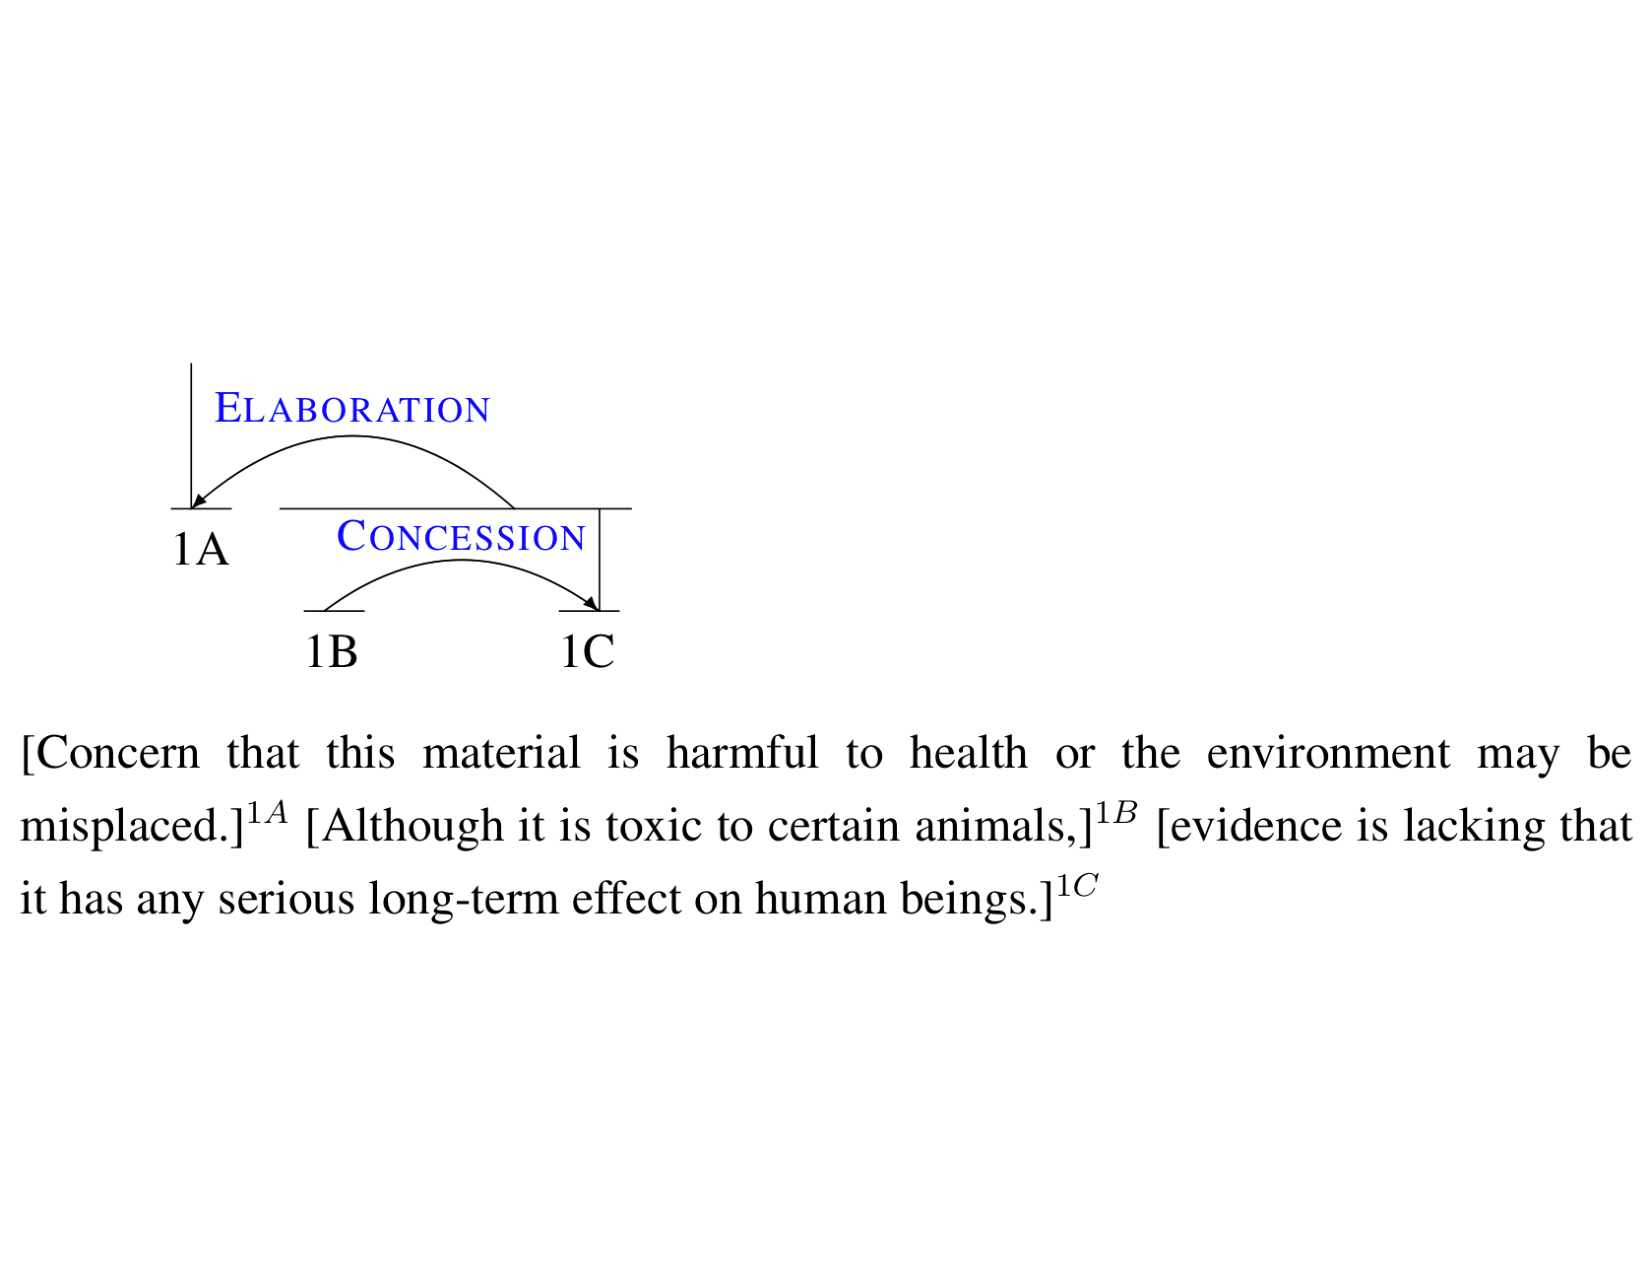
\includegraphics[width=10cm]{plots/rst-tree-1.pdf} }}%
    \qquad
    \subfloat[paratactic]{{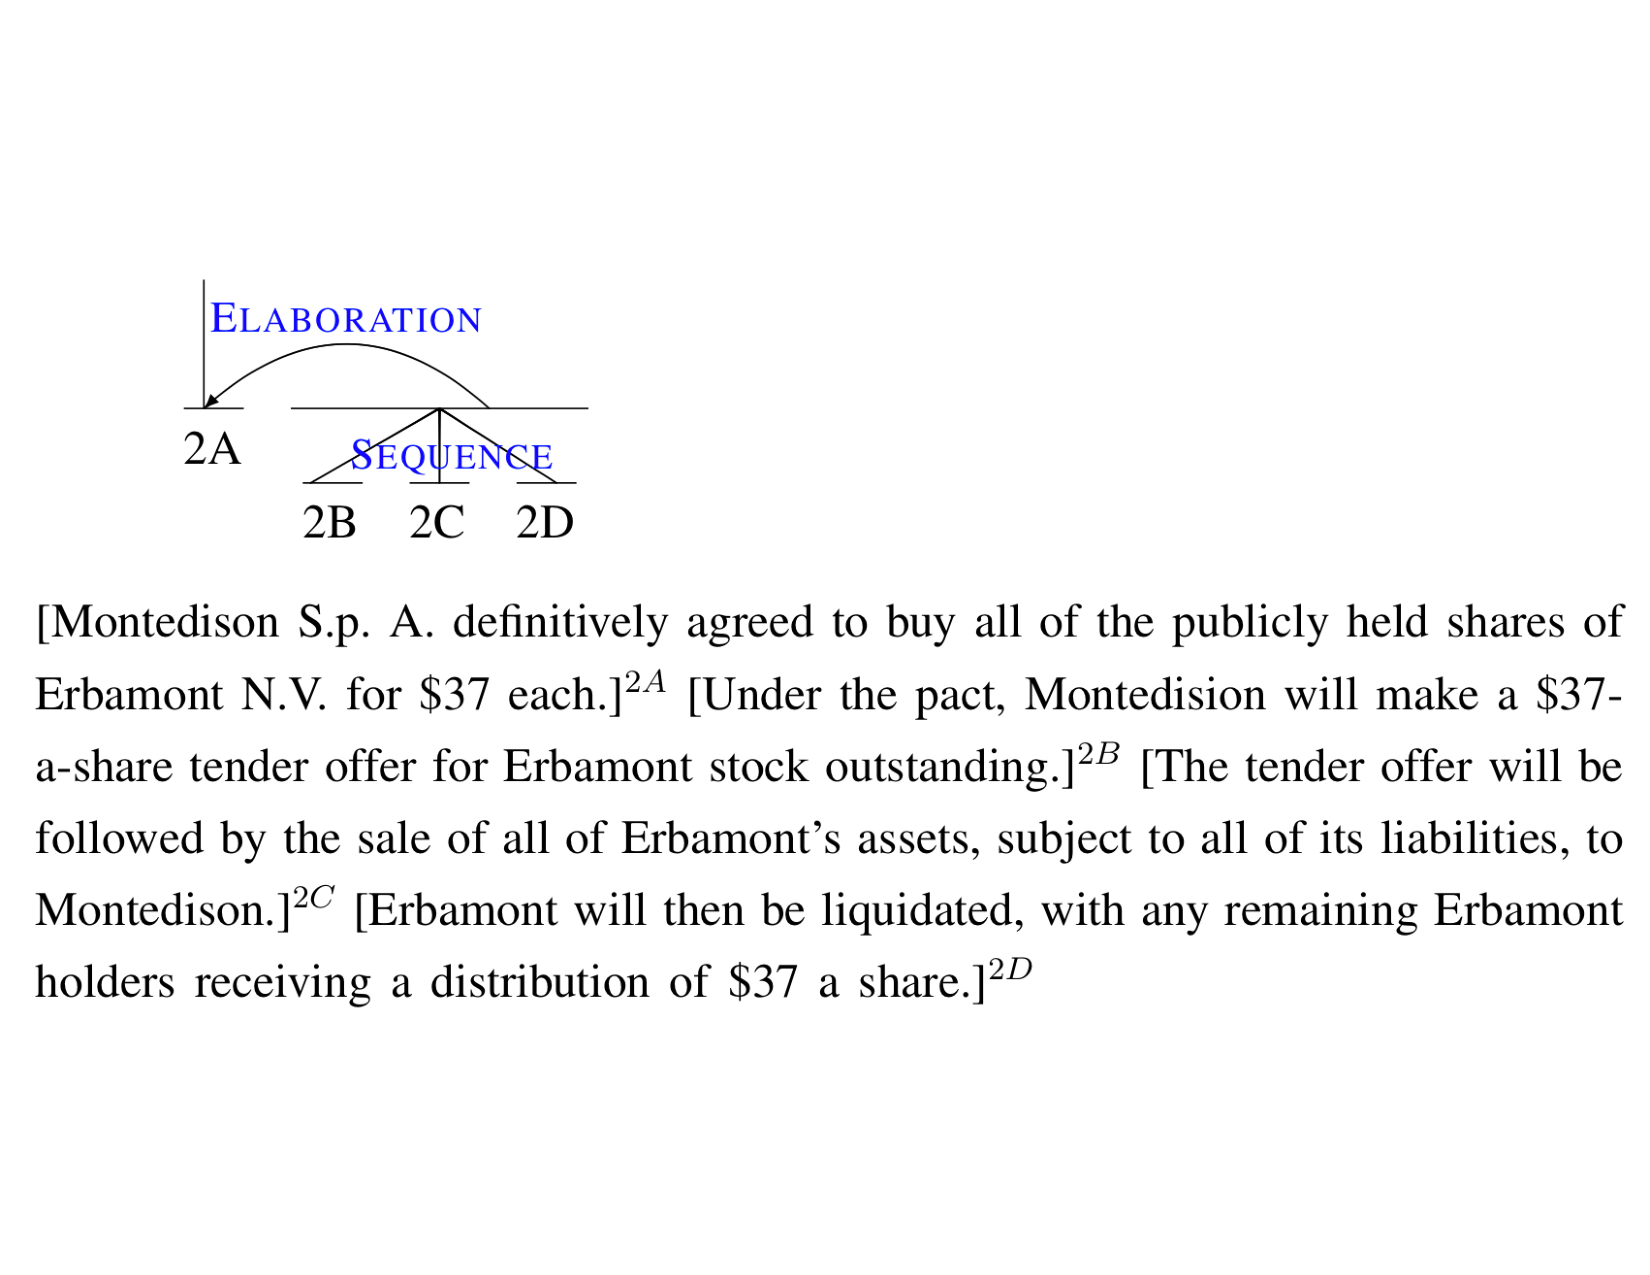
\includegraphics[width=10cm]{plots/rst-tree-2.pdf} }}%
    \caption{RST trees illustrating hypotactic and paratactic syntactic relations.}%
    \label{fig:background_rst}%
\end{figure}

%\dirrel{}
% {\rstsegment{\refr{txt1}}}{Elaboration}
% {
% \dirrel{Concession}{\rstsegment{\refr{txt2}}}
%    {}{\rstsegment{\refr{txt3}}}
% }
% \begin{rhetoricaltext}
%   \unit[txt1]{{Concern that this material is harmful to health %or the environment may be misplaced.}}
%   \unit[txt2]{{Although it is toxic to certain animals,}}
%   \unit[txt3]{{evidence is lacking that it has any serious long-term effect on human beings.}}
% \end{rhetoricaltext}
% \dirrel{}
% {
% \dirrel{}
% {
% \dirrel{}
% {
%  \dirrel{}
%  {
%   \dirrel{}
%   {\rstsegment{\refr{txt1}}}{Elaboration}
%   {\rstsegment{\refr{txt2}}}
%  }{Consequence}
%  {
%   \dirrel{}
%   {\rstsegment{\refr{txt3}}}{Elaboration}
%   {\rstsegment{\refr{txt4}}}
%  }
% }{Elaboration}
% {\rstsegment{\refr{txt5}}}
% }{Elaboration}
% {
%   \dirrel{}
%   {\rstsegment{\refr{txt6}}}{Elaboration}
%   {\rstsegment{\refr{txt7}}}
% }}{Elaboration}
% {
%   \dirrel{}
%   {\rstsegment{\refr{txt8}}}{Elaboration}
%   {\rstsegment{\refr{txt9}}}
% }

%  \begin{rhetoricaltext}
%   \unit[txt1]{{Emerson Electric Co. and Robert Bosch G.m.b. H. said the Federal Trade Commission has requested additional information from the two companies about their announced intention to acquire Vermont American Corp. for \$40 a share, or about \$440 million.}}
%   \unit[txt2]{{Yesterday, in composite trading on the American Stock Exchange, Vermont American common closed at \$39.75, off 25 cents.}}
%   \unit[txt3]{{The FTC's request was "not unusual" and Emerson will make a "full and prompt" response, according to a spokesman.}}
%   \unit[txt4]{{Spokesmen for Emerson and Vermont American, which has agreed to be acquired, said they don't anticipate "any problems" with the completion of the transaction.}}
%   \unit[txt5]{{An FTC spokesman said the matter is "in a non-public posture at this time" and declined to comment further.}}
%   \unit[txt6]{{Emerson and Bosch, through their joint acquisition arm, Maple Acquisition, have begun a cash tender offer for all of Vermont's common shares outstanding.}}
%   \unit[txt7]{{The offer, set to expire Nov. 1, may be extended pending the timing and resolution of the FTC request, the companies said.}}
%   \unit[txt8]{{St. Louis-based Emerson and Stuttgart-based Bosch make electrical and electronic products, including power tools.}}
%   \unit[txt9]{{The Vermont American acquisition is designed to enhance their position in the accessories portion of the power-tool industry.}}
%  \end{rhetoricaltext}

RST was operationalized in \newcite{Carlson:2001} with the RST Discourse Treebank (RST-DT).\footnote{\url{1https://catalog.ldc.upenn.edu/LDC2002T07}} This corpus consists of 385 Wall Street Journal articles from the Penn Treebank. Further research then proposed a set of rules to convert an RST tree into a dependency tree, where generally heads correspond to nuclear EDUs \cite{Hirao:2013}. 

With dependency trees being an appealing structure for computational models and the availability of the annotated corpus, RST has been widely adopted by the research community. In fact, RST has been shown to help with NLP tasks ranging from sentiment analysis to summarization, spanning domains such as online reviews and medical papers (\newcite{Ji:2017}, \newcite{Li:2016}, \newcite{Dacunha:2007}, \textit{interalia}). However, this same widespread use allowed the community to analyze its shortcomings, both in the theory and how it was operationalized. In our first study on discourse segmentation in the medical domain, we find evidence of problem areas for the way RST was operationalized.

\section{Structured Prediction and Attention}
\label{sec:structuredpred}
Statistical models can learn very well to detect patterns in large amounts of data. However, we also need to incorporate biases such as linguistic theories that help the model learn a task better. In this setting, the model predicts structured objects such as parse trees instead of scalars. 

With the shift to deep learning, research has focused more on models that learn latent representations of sentences or documents, constrained only by the end task. In our second study, we analyze one such model and attempt to incorporate some level of discourse theory. 

\section{Chapter Summary}

In this chapter, we described the two major concepts underpinning this report: RST and structured prediction. 



\chapter{Cross-Domain Discourse Segmentation}\label{ch:rstseg}

This chapter describes a short study on differences in automated RST discourse segmentation across two different domains (news and medical) and using two different RST segmenters. The work
in this chapter was done in collaboration with Titan Page.

Code and data for all experiments in this chapter are available here: \url{https://github.com/elisaF/cross_domain_segmentation}.

\section{Chapter Overview}

Dividing a text into units is the first step in analyzing a discourse. This first critical step is often overlooked by researchers, despite several studies showing this to be a significant source of error that propagates to the downstream tasks of span, nuclearity and relation labeling \cite{Feng:2015}. Furthermore, segmenting in a non-news domain, such as medical, has not been well studied and could present additional challenges.

In this study, we compare segmentation errors in the news versus medical domain and aim to understand the differences. Because segmentation has not been studied in the medical domain, we annotate a novel small-scale corpus. We use two different RST parsers to further understand whether the quality of the parser itself affects the error differences. Not surprisingly, the news domain outperforms the medical domain when using both segmenters. When using the higher-quality RST segmenter, we find it outperforms the poorer segmenter by a considerable margin in the news domain, but by a much smaller amount in the medical domain. Thus, we conclude that improving an RST segmenter in the news domain provides little benefit to medical. A qualitative analysis finds that the higher error rate in the medical domain is often due to idiosyncrasies found in both the news domain that the segmenter has learned, and in the medical domain that the segmenter has never seen before.

Our contributions in this work are two-fold: a small-scale corpus of medical documents annotated with RST-style discourse; a quantitative and qualitative analysis of the discourse segmentation errors in the medical domain that lay the groundwork for understanding both the limits of existing RST segmenters and problematic areas stemming from the way the RST theory was first operationalized.

\section{Motivation}
On the one hand, the segmentation task appears to be well-defined, as suggested by a high inter-annotator agreement (kappa=0.92), although this number is based on only 9 documents\footnote{Although 53 documents were doubly-annotated in the RST-DT corpus, all except 9 were \emph{pre-segmented} before being given to the annotators.} \cite{Carlson:2001}.
The best discourse segmentation results are quite high at 92.6 F1 \cite{Feng:2015}. Perhaps because of these strong results, segmentation is often dismissed as a solved task. Many RST parsers evaluate only on gold EDUs and do not include a segmenter. Nevertheless, previous studies \cite{Soricut:2003,Fisher:2007,Joty:2015,Feng:2015} identify this first step as a primary bottleneck for accurate discourse parsing. Critically, even using the best-performing segmenter degrades results by 10\% on the downstream tasks of span, nuclearity and relation labeling when using predicted instead of gold EDUs \cite{Feng:2015}.

\section{Related Work}
The challenge of evaluating a model on a domain different from where it was trained is a well-studied area of research. 
%In the area of discourse, although not using RST, \newcite{Prasad:2011} show that training on the Penn Discourse TreeBank (in the news genre) does not generalize well to a biomedical corpus for both classifying discourse connectives and discourse relations.% 
In RST, much work already recognizes differences when moving away from the news domain. \newcite{Rimrott:2007} finds that certain relation types never occur in a small-scale analysis of scientific texts. \newcite{Bachand:2014} notes systematic differences in the distribution of discourse relations between news and online reviews. 

Despite these differences, most research using RST makes no attempt to modify the news-trained parsers (or segmenters), even though they are evaluating on considerably different domains. 
For example, the text classification model in \newcite{Ji:2017} evaluates on online reviews using a news-trained RST discourse parser. We performed a small-scale study on Yelp reviews using their news-trained segmenter, and found the segmenter performance very poor. The EDU boundaries often occurred in the middle of a clause, and the EDUs themselves were often nonsensical: 2.2\% of the EDUs were a punctuation mark, 6.4\% were 1-word EDUs (such as \lit{I}, \lit{like}, \lit{really}), and 7.9\% were 2-word EDUs (such as \lit{pleasantly surprised}, \lit{completely unethical}). In fact, when corresponding with the paper authors, it was found that they did not use their own segmenter because of these issues.

Some studies do make an attempt to accommodate the different domain. For example, \newcite{Dacunha:2007} used RST to summarize medical articles, but only used a subset of the relation types that were observed to occur in that domain. However, in both cases, differences in discourse \emph{segmentation} are largely ignored.

The only study we are aware of that specifically focuses on discourse segmentation in different domains is that of \newcite{Braud:2017}. The overall aim, though, is slightly different in that their goal is to design a segmenter for under-resourced languages by relying only on part-of-speech tags. The proposed neural network model that utilizes a multi-task learning setting to train on different RST corpora is able to outperform simple baselines. However, the study makes the simplifying assumption that each RST corpus represents a single domain, which is not always accurate (the GUM corpus\cite{Zeldes:2017} spans 4 different genres-- interviews, news, travel guides, how-tos).   

\section{Experiment}
We automatically segment the 11 Wall Street Journal articles and 11 sections of medical reports using the \textsc{DPLP} segmenter \cite{Ji:2014} and the segmenter proposed in \newcite{Feng:2014}, which we refer to as \textsc{Feng}.\footnote{We choose these two segmenters as they are the most widely-used and publicly available (most RST parsers do not include a segmenter).} We evaluate the segmenter's ability to detect EDU boundaries present in the gold data (RST-DT and the novel medical corpus) using the metrics of precision, recall and F1.

\subsection{The Corpora}
\begin{table}[t]
\centering
\begin{tabular}{ccccc}
\toprule
Corpus & \#documents  & \#tokens     & \#sentences     & \#EDUs    \\ \hline \hline
\textsc{RST-DT small} &11  &4031  &166  &403  \\
                                   \textsc{Medical} & 11 &3324  &166  &385\\             \bottomrule
\end{tabular}
\caption{Corpus statistics.}
\label{tab:cross_domain_corpus}
\end{table}
The corpora statistics are summarized in Table \ref{tab:cross_domain_corpus}. The Medical corpus consists of 2 clinical trial reports from PubMed Central which were divided into their sections. Each section was manually annotated, resulting in 11 labeled documents. The News corpus was created by sampling the same number of Wall Street Journal articles from the ``Test'' portion of the RST-DT, that were similar in length to the medical documents. 

\subsection{Experimental Setup}
For the medical documents, XML formatting was stripped, and figures and tables were removed. The sections for \textit{Acknowledgements}, \textit{Competing Interests}, and \textit{Pre-publication History} were not included. For the news documents, no preprocessing was performed. 

The RST parsers, both of which employ the Stanford Core NLP pipeline \cite{Manning:2014} for preprocessing, were updated to use the same version of this software (2017-06-09). For the Feng parser, we enabled the option to perform a second pass of EDU segmentation using global features.

\begin{table}[t]
\centering
\begin{tabular}{cllll}
\toprule
\multicolumn{1}{l}{\textsc{RST Segmenter}} & \textsc{Domain}  & \textsc{F1}     & \textsc{P}     & \textsc{R}    \\ \hline \hline
\multirow{2}{*}{\textsc{DPLP}}              & \textit{News}    & 82.56 & 81.75 & 83.37 \\
                                   & \textit{Medical} & 75.20 & 77.26 & 73.25 \\ \hline
\multirow{2}{*}{\textsc{Feng}}              & \textit{News}    & \textbf{95.72} & \textbf{97.19} & \textbf{94.29} \\
                                   & \textit{Medical} & 78.95 &80.00 & 77.92 \\ \bottomrule
\end{tabular}
\caption{Performance of discourse segmentation using two different discourse segmenters and evaluated on two different domains.}
\label{tab:cross_domain_f1}
\end{table}

\section{Results}
Table \ref{tab:cross_domain_f1} lists our results. As expected, the \textit{News} domain outperforms the \textit{Medical} domain, regardless of which segmenter is used. In the case of the \textsc{DPLP} segmenter, the gap between the two domains is about 7.4 F1 points. Note that the performance of this segmenter on \textit{News} lags considerably behind the state of the art (-10 F1 points). When switching to the \textsc{Feng} segmenter, the performance on \textit{News} increases dramatically (+13 F1 points). However, the performance on \textit{Medical} increases by a mere 3.75 F1 points. Thus, large gains in \textit{News} translate into only a small gain in \textit{Medical}, underscoring the need to handle out-of-domain data.

\subsection{Error Analysis}
We perform an error analysis to understand the types of errors present in both domains, and contrast with those seen only in the \textit{Medical} domain. We analyze errors only in the better-performing \textsc{Feng} segmenter.

Across both domains, the segmenter has trouble with infinitival clauses which are generally not treated as separate EDUs but the guidelines contain several nuanced exceptions. In the following example, the first infinitival clause is not separated because it is a complement of the verb, while the second is segmented as a modifier to the preceding noun phrase \lit{its attempt}: 
\begin{quote}
[U.S. Memories is seeking major investors \textit{\textbf{to} back its attempt}][\textit{\textbf{to} crack the \$10 billion market $\ldots$}]
\end{quote}
Interestingly, \newcite{Braud:2017} also found this to  be a large source of errors for their segmentations. 

\begin{table}
  \hfill
  \begin{minipage}{\textwidth}
  \centering
  \begin{maybesmall}
\begin{tabular}{lp{5.5cm}p{5.5cm}}
\toprule
\textsc{Error Type}    & \textsc{Predicted}     & \textsc{Gold} \\ \hline\hline
\multicolumn{1}{l}{\lit{in} modifier} & {[}compare the safety of hydrochloride \emph{in} patients{]}{[}diagnosed with{]}            & {[}compare the safety of hydrochloride{]}{[}\emph{in} patients{]}{[}diagnosed with{]}        \\ \hline
past verb                           & {[}Ten patients{]}{[}\emph{dropped} out of{]}                                               & {[}Ten patients \emph{dropped} out of{]}                                                    \\ \hline
title                               & {[}\emph{Conclusion} The offer of a prize draw incentive{]}                                    & {[}\emph{Conclusion}{]}{[}The offer of a prize draw incentive{]}                               \\ \hline 
dash                                & {[}(95 \% CI 0.96{]}{[}\emph{--} 1.13){]}                                                      & {[}(95 \% CI 0.96 \emph{--} 1.13){]}                                                           \\ \hline
citation*                            & {[}Studies have shown either small increase in response{]}{[}\emph{\{6\}} or more rapid{]} & {[}Studies have shown either small increase in response \emph{\{6\}}{]}{[}or more rapid{]} \\ \bottomrule
\end{tabular}
 \end{maybesmall}
  \end{minipage}
\caption{Types of segmentation errors in the \textit{Medical} domain with examples of predicted and gold EDU boundaries marked in square brackets (*the square brackets for the citation were changed to curly brackets to avoid confusion with EDU boundaries).}
\label{tab:cross_domain_errors}
\end{table}

In the \textit{Medical} domain, Table \ref{tab:cross_domain_errors} summarizes and gives example of the most frequent errors. The first group of errors can be attributed to differences in syntactical constructions. The segmenter has trouble identifying embedded EDUs, in particular modifiers starting with \lit{in} describing the circumstance or background. Although \lit{in} phrases occur often in \textit{News}, they usually refer to a location or time (e.g., \lit{offices \emph{in} New Orleans}). For many clauses with past tense verbs, an EDU boundary is surprisingly inserted between the subject and verb. The segmenter is likely confusing these cases for participial phrases that modify the noun, which would be treated as embedded EDUs (e.g., \lit{[the charge][\textit{related} to the action]}). Because this analysis partly relies on syntax, a source of this error could be traced back to the Stanford Core NLP parser, which is also trained on news articles. 

The next group of errors relate more to differences in formatting and markup of the two domains. The section titles in the \textit{Medical} domain are invariably never detected by the segmenter. Although \textit{News} contains headers, they are always separated by a colon. Punctuation is a strong and easy signal for EDU boundaries. Although even punctuation can be ambiguous and conflicting across domains. While the em dash (\lit{--}) is typically used in the same context as parentheses or commas, we find cases in the \textit{Medical} domain where it is used as a hyphen or en dash (\lit{-}), for example to specify a numerical range. Finally, the last error is one that would be common in many scientific domains. Citations do not occur in \textit{News}, and the square brackets around citations used by PubMed Central articles are confusing to the segmenter.

\section{Chapter Summary}
As a first step in understanding discourse differences between domains, we analyze the performance of two discourse segmenters on \textit{News} and \textit{Medical}. For this purpose, we create a first, small-scale corpus of annotated medical documents. We find that both discourse segmenters perform better on \textit{News}, as expected. However, we also find that large improvements in the \textit{News} domain gained by using a better segmenter do not translate into substantial improvements in the \textit{Medical} domain. An error analysis reveals difficulty in both domains for cases requiring a fine-grained syntactic analysis, as dictated by the RST-DT annotation guidelines. This finding suggests a need for either a clearer distinction in the guidelines, or more training examples for a model to learn to distinguish them. In the \textit{Medical} domain, we find that differences in syntactic construction and formatting, including use of punctuation, account for most of the segmentation errors. We hypothesize syntactic errors can be partly traced back to syntactic parsers used in the preprocessing steps that are also trained on news.

Addressing even one of these issues may yield a multiplied effect on segmentation improvements as this domain is by nature highly repetitive and formulaic. However, a future avenue of research would be to first understand what impact these segmentation errors have on downstream tasks. On the one hand, using RST trees generated by the lower-performing \textsc{DPLP} parser nevertheless provides small gains to text categorization tasks such as sentiment analysis \cite{Ji:2017}. On the other hand, understanding the verb form, which proved to be difficult in the \textit{Medical} domain, has been shown to be useful in distinguishing text on experimental results from text describing more abstract concepts (such as background and introductory information) \cite{deWaard:2012}.


\chapter{Latent Discourse Structures}
\label{ch:latent}

This chapter focuses on latent discourse structures that are learned by a neural network, in contrast to the first chapter that examined explicit structures as dictated by a linguistic theory (RST). 

Code and data for all experiments in this chapter are available here: \url{https://github.com/elisaF/structured}.

\section{Chapter Overview}
Neural networks have seen considerable success in learning latent representations for linguistic constructs ranging from syntax to discourse \cite{Choi:2017,Yogatama:2017,Liu:2018}. However, more recent work calls into question what the models are actually learning, finding they are not consistent with any linguistic theory \cite{Williams:2017}. At the same time, these questions are spurred by the research community's desire to understand neural networks at a deeper level, instead of treating them as black boxes.

We find the \newcite{Liu:2018} model to be an excellent starting point for addressing these questions in regards to discourse and latent representations of documents. This model employs structured attention that is parsed into a non-projective dependency tree. Analyzing the attention weights and resulting tree allows us a window into the network. We utilize this model to perform an in-depth analysis to understand what the model is learning and whether the structured attention can be interpreted as discourse. 

Our analysis and experiments on different inputs to the model show that the structured attention is mostly attending to a single sentence, the root of the dependency tree, which contains lexical cues useful for the task. The model is not learning discourse and the derived trees do not resemble those of any discourse theory. We propose a variant of the model that induces deeper latent structures.

Our contributions in this work are two-fold: we present a comprehensive analysis of the \newcite{Liu:2018} model that reveals what the model is learning and refute the claim that these latent structures represent discourse. Secondly, we propose a variant of the model that is able to learn deeper structures.

\section{Related Work}
We first describe the \newcite{Liu:2018} model, which we analyze and propose a variant of. We next discuss the growing area of research into understanding representations induced by neural networks.

\smallskip
\noindent\textbf{Structured Attention}
Attention has gained widespread adoption as a way to selectively focus on parts of the input, which is particularly useful in models such as recurrent neural networks that do not handle long inputs well \cite{Luong:2015}. Structured attention is then introduced as a way to learn unsupervised latent representations. \newcite{Kim:2017} use graphical models to induce hidden representations that are able to outperform models using simple attention on a variety of tasks. Importantly, they find the attention distributions of the learned structures to be interpretable and intuitive to the given task. In a similar vein, \newcite{Liu:2018} learns a structured attention that can be parsed as a non-projective dependency tree. We describe this model in more detail as we choose to analyze this model in our study.

The \newcite{Liu:2018} model consists of both sentence-level and document-level attention. The underlying attention is the same, but operates on different input. At a high level, the sentence-level model composes words into a single representation of a sentence. These sentence representations are then composed into a single representation of a document in the document-level model. In the sentence-level model, a bidirectional LSTM is run over a sentence, and these hidden representations $[h_1 , h_2 , \ldots, h_n]$ are used as the representations for the words in the sentence. They further decompose this output into a semantic part ($e_t$) and a structure part ($d_t$):
\begin{equation}
[e_t, d_t] = h_t
\end{equation}
They then use the Matrix Tree algorithm to calculate the marginal probabilities, or \emph{attention scores}, $a_{ij}$ using the structure vectors $\boldsymbol{d}$. The attention is parsed into probabilities over a non-projective dependency tree.  The semantic part of a word is then updated with attention by first calculating a context for all the possible parents of that word as follows:
\begin{equation}
\label{eq:parent}
p_i = \sum^{n}_{k=1}a_{ki}e_{k} + a^r_i e_{root}
\end{equation}
where $a_{ki}$ is the probability that $k$ is the parent of $i$, $e_k$ is the semantic vector of the parent, $e_{root}$ is a special embedding for the root node, and $a^r_i$ is the attention score for the $i$-th word being the root. 

The parent vectors are then concatenated to the semantic vectors and passed through a non-linear function, resulting in the \emph{updated} semantic vector $r_i$. While \newcite{Liu:2018} describes additionally concatenating a vector for all possible children $c_i$ as illustrated in \ref{eq:update_liu}, their code only makes use of the parent vectors as in \ref{eq:update}.

\begin{equation}
\label{eq:update_liu}
*r_i = tanh(\boldsymbol{W_r}[e_i, c_i, p_i])*
\end{equation}
\begin{equation}
\label{eq:update}
r_i = tanh(\boldsymbol{W_r}[e_i, p_i])
\end{equation}
where $\boldsymbol{W_r}$ are weights learned by the network.

Finally, a max pooling layer produces the final sentence representation $v_i$. Note that this pooling strategy chooses just \emph{one} representation of a word (or \emph{one} sentence for the document-level model) . This could prove detrimental to capturing a representation of the entire sentence (or entire document). The document-level model employs the same attention mechanism, but takes as input the outputs of the sentence-level model. That is, a biLSTM is run over the sentence representations $[v_i, \ldots, v_n]$ to yield a document representation $q_i$. At test time, the Chu-Liu-Edmonds algorithm is used to derive the maximum spanning tree over these attention scores.\footnote{We use the implementation in \url{https://github.com/atofigh/edmonds-alg.git}.}

\smallskip
\noindent\textbf{Interpreting latent structures} Upon the heels of a surge in neural networks and attention, a large part of the community is now striving to understand what these structures represent. For example, \newcite{Williams:2017} examines latent parse trees learned by two neural network models. They find that while the models perform very well, the learned trees are shallower than their explicitly parsed counterparts (PTB parses) and do not resemble any linguistic theory. Our study finds similar results when interpreting document-level trees and comparing them to discourse parses. 

Several papers have also proposed toy datasets of mathematical operations to understand how models are composing functions and gage their ability to produce a plausible tree \cite{Hupkes:2017,Nangia:2018}. \newcite{Hupkes:2017} in particular propose \lit{diagnostic classifiers} to test hypotheses on what the hidden representations are encoding. While we find this research worthwhile and engaging, we feel that in order to meet our goal of understanding discourse and its latent representations, we need real-world data.

\section{Models}
In this chapter, we first explain our choice of model, and then describe our proposed variants of the \newcite{Liu:2018} model.

\subsection{Model Choice: Latent or Explicit?}
Models such as \newcite{Liu:2018} attempt to learn a \emph{latent} structure for a document, while models such as \newcite{Ji:2017} dictate an \emph{explicit} structure, namely RST discourse dependency trees. While it would be desirable to compare and contrast both models, we were not able to replicate the performance of \newcite{Ji:2017}. Despite using their publicly available code on the same dataset (Yelp 2015), our accuracy on their \emph{full} model (that uses RST trees) never exceeded 65.1, a considerable gap from the reported 71.8. Upon inspection of the parsed discourse trees, we noted very poor EDU segmentation. After corresponding with the authors, we learned they in fact did not use their own discourse segmenter, as reported in the paper. We thus attempted to reproduce their results first using sentences (parsed by Stanford Core NLP \cite{Manning:2014}) and then using the best-performing RST segmenter \cite{Feng:2014}. In both cases, the results were equally low. Suspecting that bad RST trees were the culprit, we tried to reproduce the results of their baseline \emph{additive} model, which effectively runs a bidirectional LSTM over just the EDUs, without taking into account the tree structure. Accuracy approached 64.0, still a far cry from the reported 68.5.  Finally, because tuning the model was very slow on dyNet \cite{dynet}, we reimplemented the \emph{additive} baseline model in PyTorch \cite{pytorch}, and the results were still the same. Because of the consistently negative results, we decided not to pursue this model and instead focus on latent structures by exploring the model in \newcite{Liu:2018}. 

\subsection{Model Variants}
We propose several variants of the \newcite{Liu:2018} model  first by modifying its inputs, and finally by modifying its architecture.

\smallskip
\noindent\textbf{baseline} The baseline model uses the publicly available code for \newcite{Liu:2018} with both sentence- and document-level attention. 

\smallskip
\noindent\textbf{root-only} The aim of this model is to understand how much the original model relies only on root sentences in the learned dependency tree. For all documents in the corpus, we remove all sentences that are not attached to the root. We then create new embeddings and retrain the \textbf{baseline} model on the pruned corpus.

\smallskip
\noindent\textbf{edu} This model attempts to inject explicit structure into the network. Specifically, we feed in EDUs instead of sentences into the \textbf{baseline} model.\footnote{We do not take the route of modifying the word inputs into EDUs, as RST structures do not always result in trees that can be isolated into a single sentence. That is, it is possible for only one segment of a sentence to attach to another sentence \cite{vanderVliet:2011}} We hypothesize this modification will encourage deeper structures as composition might be required to reconcile conflicting sentiments that exist at a finer-grained level than sentences as noted in \newcite{Socher:2013} (e.g., \lit{[The potato and mushrooms were good,][but the green beans were way to ``Al Dente'']}).
For segmenting the text, we use \newcite{Feng:2014} with global features, which obtains the best segmentation on RST-DT. 

\smallskip
\noindent\textbf{deeper} This model attempts to encourage deeper tree structures by making three changes to the original model: incorporating the updated semantic vectors from \emph{subtrees} into the final tree representation, removing the document-level biLSTM, and using a different function at the pooling layer. 

First, recall in \ref{eq:update_liu} that the semantic vector $r_i$ is updated with the probabilities of possible children $c_i$. However, this update only takes into account direct children, not the integrated information from a whole \emph{subtree}. To further percolate information from subtrees, we propose an additional update to the semantic vector. Starting from the original updated semantic vector:
\begin{equation}
r_i = tanh(\textbf{W}_r[e_i, c_i])
\end{equation}
we then propose a new representation for the children that incorporates the above semantic vector $r_i$:
\begin{equation}
c_i^{(2)} = \sum^n_{k=1}a_{ik}r_i
\end{equation}
This new child representation is then incorporated into a new semantic vector:
\begin{equation}
r_i^{(2)} = tanh(\textbf{W}_r[e_i, c_i^{(2)}])
\end{equation}

The second modification is to remove the document-level bidirectional LSTM. We believe the learned structures are shallow because context is already incorporated by the biLSTM without any need for deeper structures. As we discuss in section \ref{sec:latent_learned}, this hypothesis is further confirmed by results on our earlier proposed model \emph{root-only}. 

Finally, we believe the max-pooling layer encourages the model to just choose one sentence, ignoring the learned structure. Instead, we propose a sum that is weighted by the probability of a given sentence being the root, that is using the learned attention score $a_i^r$:
\begin{equation}
q_i=\sum_{i=1}^n a_i^r r_i^{(2)}
\end{equation}



\section{Experiments}
We use the model with both sentence- and document-level structured attention as described in \newcite{Liu:2018} on a subset\footnote{We do not evaluate on IMDB reviews or Czech reviews because the task of sentiment analysis is already analyzed in Yelp, and we are not focused on the non-projectivity of trees.} of their same document classification tasks: sentiment analysis and Congressional vote prediction. We additionally evaluate on the task of identifying high-quality writing. 

\subsection{The Corpora}
Table \ref{tab:latent_corpora} summarizes the statistics for the three datasets we use on the document classification tasks. We describe each in more detail below. 

\begin{table}[t]
\centering
\begin{tabular}{lllllll}
\toprule
                    &         & \multicolumn{4}{c}{Number of documents}  &             \\ \cline{3-6}
Dataset             & Classes & Total & Train & Dev & Test    & Vocab. \\ \hline\hline
Yelp 2017           & 5       & 1.1M  & 914,525  & 101,615     & 100K & 131K        \\
Congressional votes & 2       & 1.7K  & 1,175    & 113         & 411     & 7.4K        \\
Writing quality     & 2       & 8.5K  & 6,806    & 850         & 850     & 48.6K       \\ \bottomrule
\end{tabular}
\caption{Statistics for the datasets used in the text classification tasks. The vocabulary size is calculated after preprocessing.}
\label{tab:latent_corpora}
\end{table}

\smallskip
\noindent\emph{Yelp 2017} We construct a dataset of 1.1M Yelp reviews from the Yelp 2017 Dataset Challenge, consisting of business reviews with a rating on a scale of 1 (negative) to 5 (positive) that we use as labels for our sentiment classification task. The data is split into roughly 80/10/10 for training, development and test. The reviews are balanced by rating in each partition. The review text is split into sentences using the Stanford Core NLP.


\smallskip
\noindent\emph{Congressional Votes} This corpus consists of speech segments from Congressional floor debates that are labeled with how the speaker voted on a given bill (\lit{yea} or \lit{nay}). We use the same dataset as \newcite{Liu:2018}, which is the preprocessed version from \newcite{Yogatama:2014}. 


\smallskip
\noindent\emph{Writing Quality} This corpus was created by \newcite{Louis:2013} and consists of science articles from the New York Times that are labeled as either \lit{very good} or \lit{typical}. The \lit{very good} class was created by using as a seed the 63 articles in the New York Times corpus \cite{Sandhaus:2008} deemed to be high-quality writing  by a team of expert journalists. The class was then expanded by adding all other science articles in the NYT corpus that were written by the seed authors (4,253 articles). For the \lit{typical} class, science articles by all other authors were included (19,520). Because the data is very imbalanced, we undersample the \lit{typical} class to be the same size as the \lit{very good}. We split this data into 80/10/10 for training, development and test, with both classes equally represented in each partition. Sentences are split using Stanford Core NLP.

\subsection{Experimental Setup}
We follow the same preprocessing steps as in \newcite{Liu:2018} except for the \emph{Writing Quality} dataset, we change the default maximum sentence length from 60 to 100 so that we discard 9\% instead of 35\% of the data. For training, we follow the same procedure with two modifications. First, we use different dimensions for the semantic and structure vectors which were found to perform slightly better (100 and 50, respectively, instead of the reported 75 and 25). Second, we critically do not batch at test time in order to accurately predict the maximum spanning tree. The code does not account for masking and therefore would not create a correctly sized tree for the shorter documents in a batch (during training, this problem is mitigated by batching with size 32 and grouping sentences of similar length into the same batch).

\section{What is learned, and is it discourse?}
\label{sec:latent_learned}
In this part of our study, we aim to understand what the \textbf{baseline} model is learning about a given  task by analyzing the latent structures, and whether these can be interpreted as discourse. We evaluate on the three described text classification tasks. We first analyze the attention scores to understand the distribution of probabilities for children and parents in the dependency tree (e.g., does the model definitively choose one child, or are probabilities spread out across all children?). We then derive the dependency tree from the learned attention scores (using the Chiu-Liu-Edmonds algorithm) that we liken to an RST discourse dependency tree. Next, we calculate statistics on these trees and perform a qualitative analysis to conclude these structures in fact do not represent discourse. Instead, the model seems to focus mainly on lexical cues.

\begin{table}[t]
\centering
\begin{tabular}{lllll}
\toprule
Model &Yelp 2013 &Yelp 2017 &Congressional votes &Writing quality \\\hline \hline 
baseline &68.1 & 71.24 & 77.27 & 83.46 \\
\bottomrule
\end{tabular}
\caption{Accuracy on the three classification tasks using the baseline \newcite{Liu:2018}.}
\label{tab:latent_accuracy}
\end{table}

Table \ref{tab:latent_accuracy} summarizes the accuracy results on the \textbf{baseline} model. We first evaluate on Yelp 2013 \cite{Tang:2015} to confirm we are able to reproduce, within reason, the performance of \newcite{Liu:2018} (they report an accuracy of 68.6). While there is no prior work on Yelp 2017, the performance is consistent with previous year datasets, though slightly higher as can be expected with a larger dataset. Our performance on the Congressional Votes marginally exceeds that reported in \cite{Liu:2018}. For the Writing Quality, while we cannot directly compare our numbers with those reported in \newcite{Louis:2013},\footnote{They used a different sampling technique and performed cross-fold validation that would not work in this setting.} we confirm our performance is very similar.

Now that we have ensured the models are indeed learning the task well, we can confidently claim the latent structures paint an accurate picture of how a document is represented. We first examine the attention weights to understand how certain the model is about this representation. Recall the structured attention is parsed as a dependency tree. The attention weights are thus a square $n\times n$ matrix where $n$ is the number of sentences, and an extra column is added at the beginning for the root symbol. For a given cell $a_{ij}$, its value represents the probability that $i$ is a child of $j$. For example, $a_{11}$ gives the probability of the first sentence attaching to the root.

\smallskip
\noindent\textbf{Attention Scores} Here we describe patterns observed for the attention scores on each of the tasks. Tables \ref{tab:latent_sentiment}, \ref{tab:latent_votes} and \ref{tab:latent_writing} illustrate the attention scores as a heat map for a test sentence. The sentences were chosen to be representative of patterns seen in each dataset. 

For Yelp, the model often chooses a sentence with strong sentiment-bearing words as the root, and then the remaining sentences attach to that sentence. The probabilities are peaked, indicating the model is considerably certain about the structure. The trees decidedly do not represent discourse, and the model instead seems to focus on lexical cues.

In the case of Congressional Votes, the structures were similarly shallow, choosing the root to be the sentence where a speaker declares their position for or against the bill. However, the probabilities were more distributed across different sentences. This could be due to the nature of the data, or more likely due to the much smaller size. In this case as well, we do not deem these structures to be representing discourse and instead the model again seems to be learning lexical items.

For Writing Quality, the structures are considerably different. Multiple root sentences are usually chosen with often a deeper tree. We do not constrain the tree to have a single head, since multi-headed RST discourse dependency trees are possible (although not as common). However, the multiple roots found in these structures do not correspond to multi-nuclear relations. Interestingly, the probabilities for the root are concentrated on sentences at the beginning of the document, although the model has no notion of order. It is less clear whether this structure could be construed as discourse, although it is decidedly not similar to RST. 

% \begin{table}[h!]
%      \begin{center}
%      \begin{tabular}{ p{5cm}  p{5cm}  p{5cm}  }
%      \toprule
%       my.Lboro & Advantages & Disadvantages \\ 
%     \cmidrule(r){1-1}\cmidrule(lr){2-2}\cmidrule(l){3-3}
%      \raisebox{-\totalheight}{\includegraphics[width=0.3\textwidth, height=50mm]{plots/Figure_1.pdf}}
%       & 
%       \raisebox{-\totalheight}{\includegraphics[width=0.3\textwidth, height=50mm]{plots/Figure_1.pdf}}
%       & 
%       \raisebox{-\totalheight}{\includegraphics[width=0.3\textwidth, height=50mm]{plots/Figure_1.pdf}}
%       \\ 
%       \begin{enumerate}[topsep=-5pt, noitemsep]
%       \item I have to say that I am very happy with my recent visit to Just Brakes
%       \item Up to date information
%       \item Fulfil students needs and wants \ldots
%       \end{enumerate}
%       & \begin{enumerate}[topsep=-5pt, noitemsep]
%       \item Accessibility
%       \item Up to date information
%       \item Fulfil students needs and wants \ldots
%       \end{enumerate}
%        & \begin{enumerate}[topsep=-5pt, noitemsep]
%       \item Accessibility
%       \item Up to date information
%       \item Fulfil students needs and wants \ldots
%       \end{enumerate}\\
%       \bottomrule
%       \end{tabular}
%       \caption{my.Lboro Analysis}
%       \label{tbl:myLboro}
%       \end{center}
%       \end{table}

\begin{table}[h!]
     \begin{center}
     \begin{tabular}{c}
     \toprule
     \raisebox{-\totalheight}{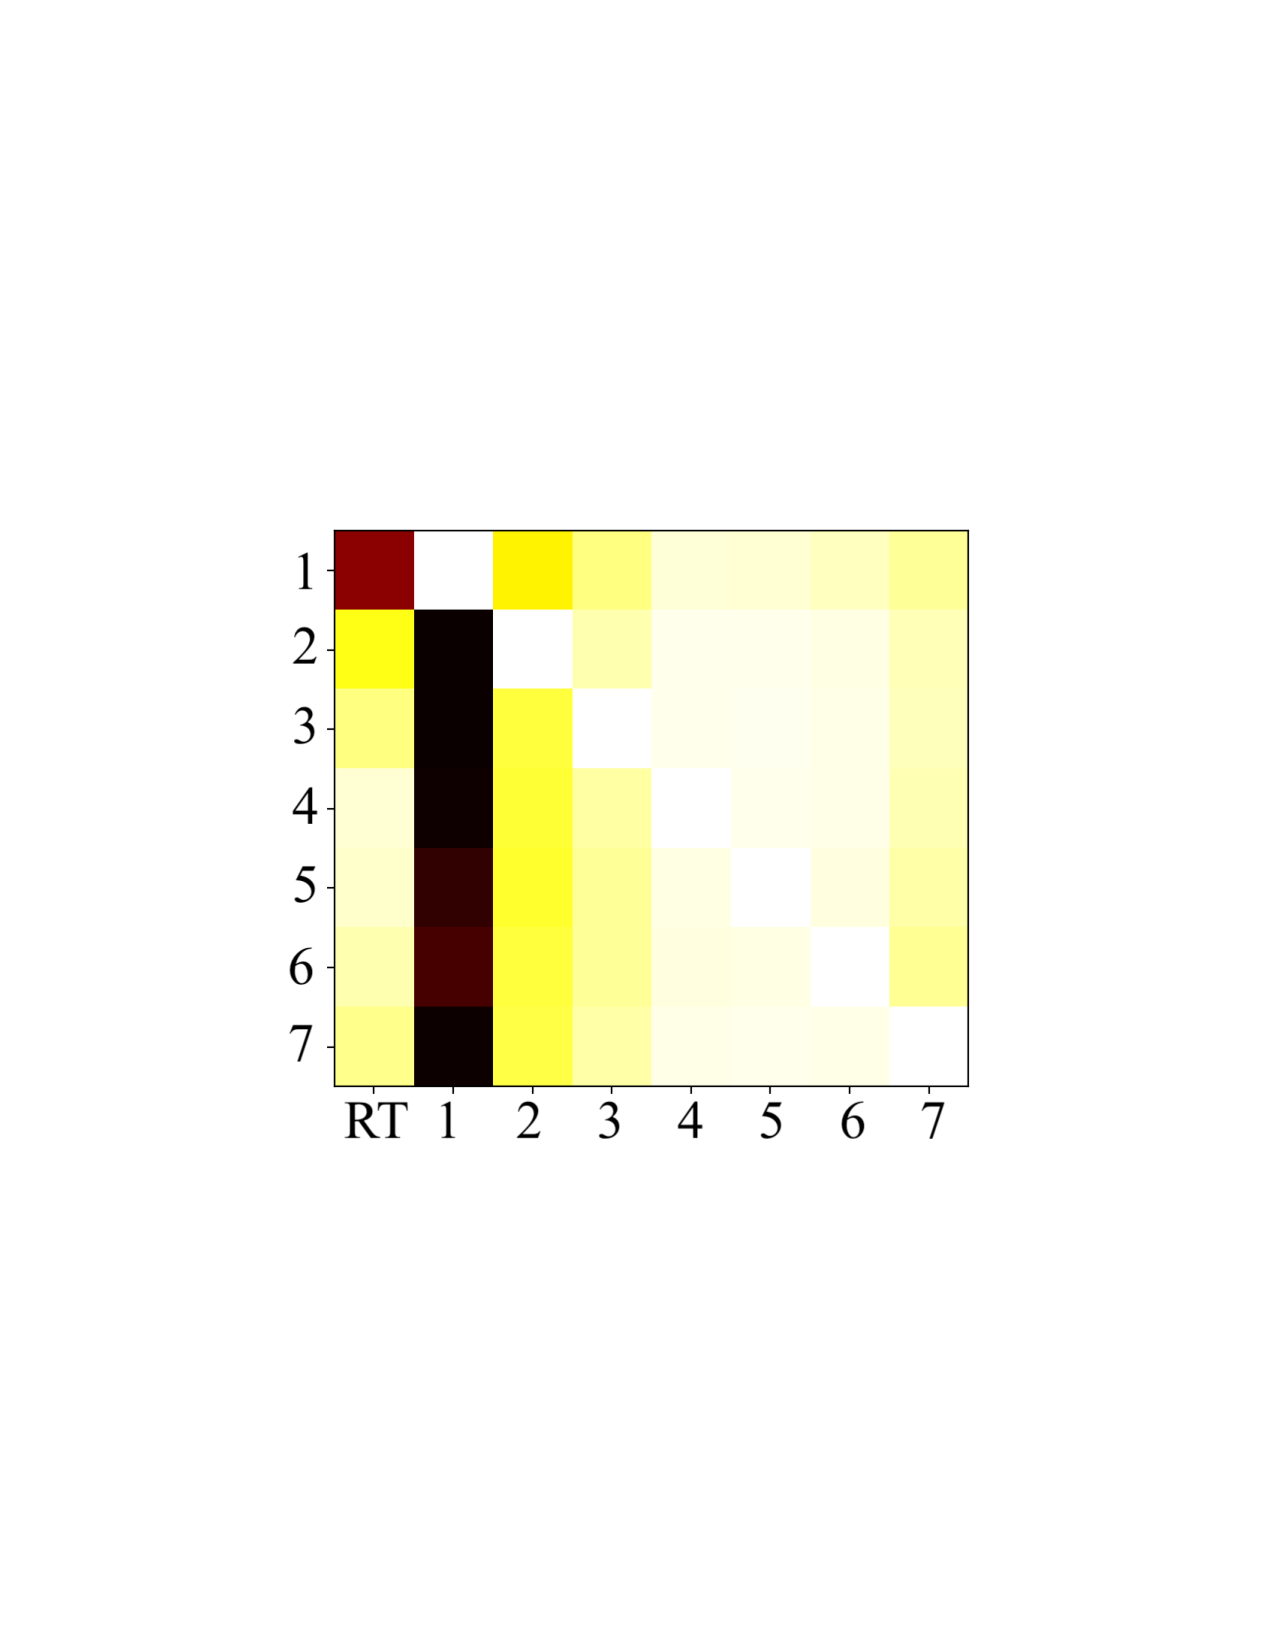
\includegraphics[width=0.4\textwidth, height=50mm]{plots/heatmap_sentiment.pdf}}\\
     \\
     \multicolumn{1}{p{15cm}}{Dependency tree: RT: [1], 1: [2, 3, 4, 5, 6, 7]} \\
     \multicolumn{1}{p{15cm}}{
      \begin{enumerate}[topsep=-5pt, noitemsep, leftmargin=*]
      \item \uline{I have to say that I am very happy with my recent visit to Just Brakes}
      \item We needed our rear brakes replaced and I forgot that we used Just Brakes for our last repair and part of our service was still under warranty
      \item The mechanic explained what we needed done and showed us the worn parts 
      \item My wife asked about an additional repair another shop said we needed , which they quoted at over 1400 
      \item Our Just Brakes mechanic said we did not need the repair 
	  \item So I assume the other shop is dishonest or incompetent
      \item Either way , thank you Just Brakes , you have earned a loyal customer 
      \end{enumerate}}\\
      \bottomrule
      \end{tabular}
      \caption{Example of attention scores, derived dependency tree and text for a test sentence in Yelp 2017 (gold label=5). Root sentences are underlined. In this example the very light and very dark shadings suggest the model is very certain about the structure.}
      \label{tab:latent_sentiment}
      \end{center}
      \end{table}

\begin{table}[h!]
     \begin{center}
     \begin{tabular}{c}
     \toprule
     \raisebox{-\totalheight}{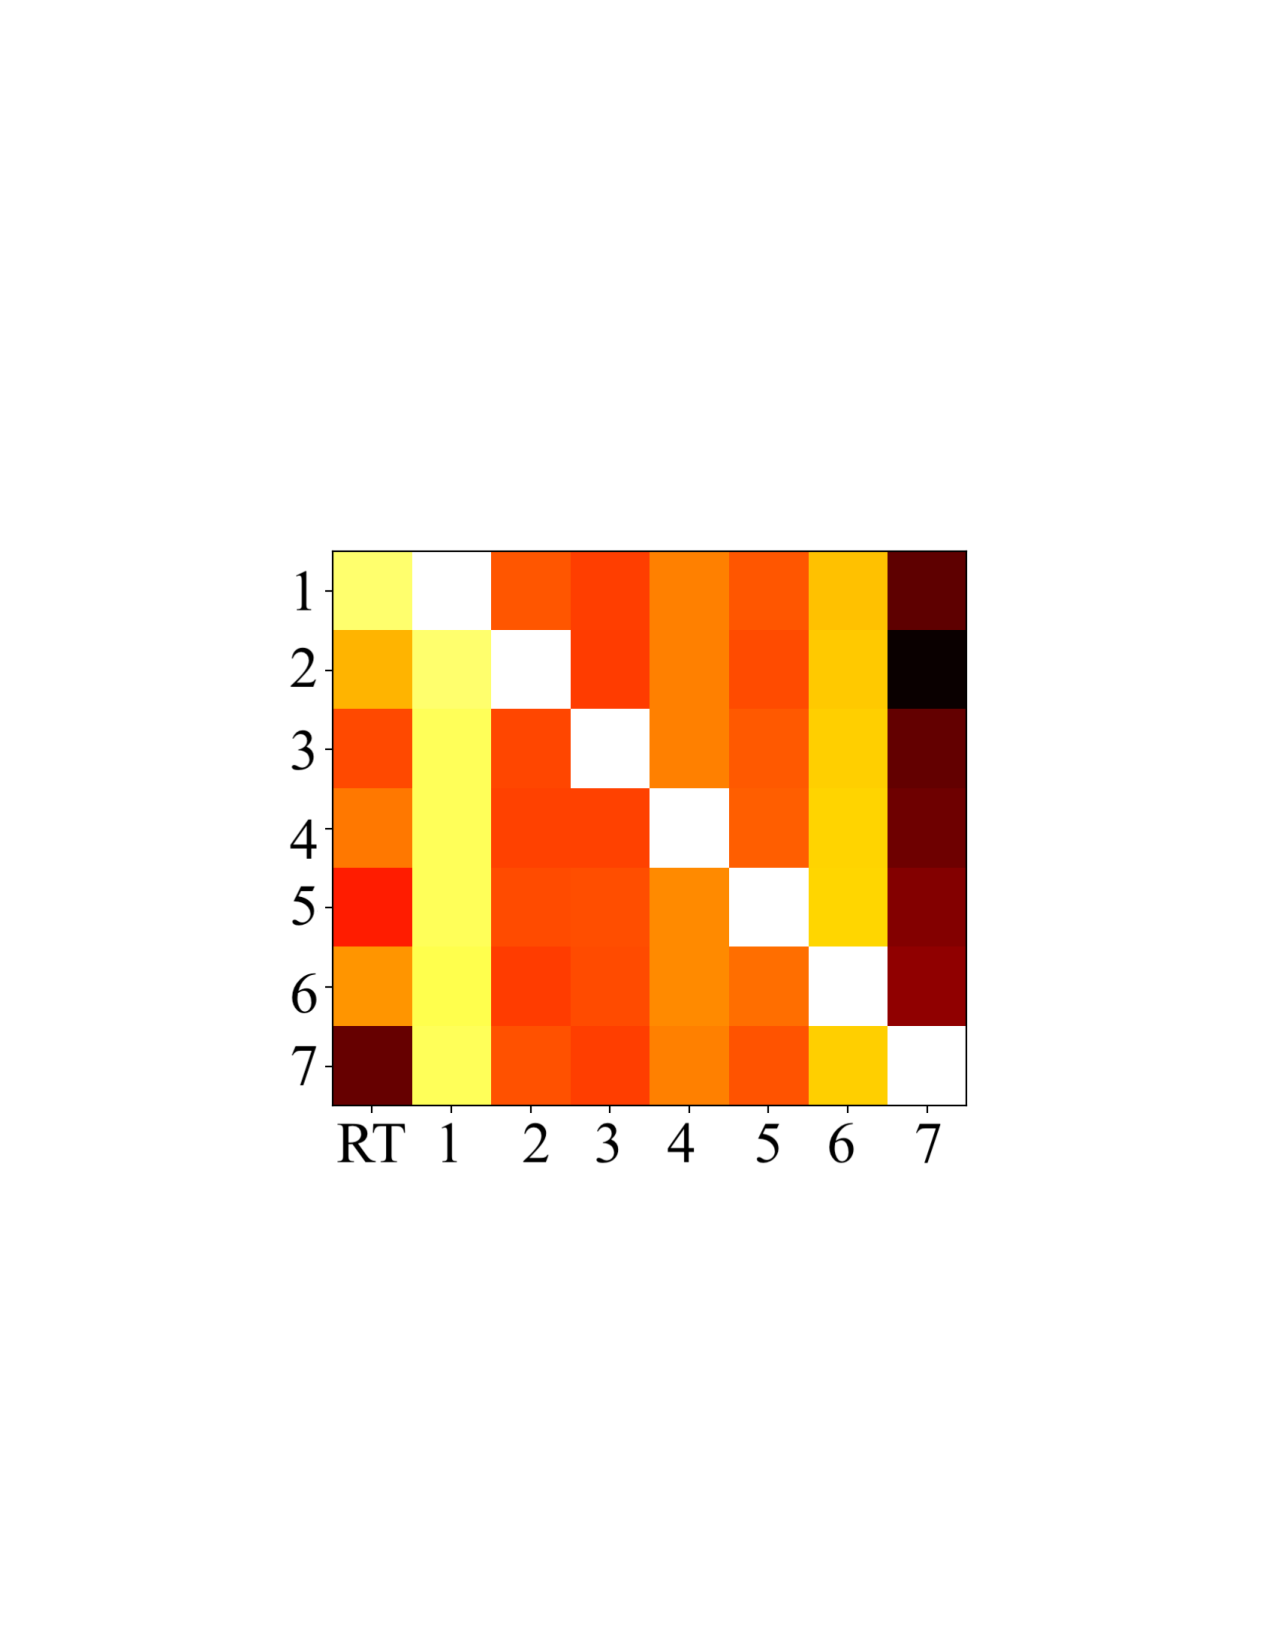
\includegraphics[width=0.4\textwidth, height=50mm]{plots/heatmap_votes.pdf}}\\
     \\
     \multicolumn{1}{p{15cm}}{Dependency tree: RT: [7], 7: [1, 2, 3, 4, 5, 6]} \\
     \multicolumn{1}{p{15cm}}{
      \begin{enumerate}[topsep=-5pt, noitemsep,leftmargin=*]
      \item madam speaker , i thank the gentleman from the great city of UNK , massachusetts , for yielding
      \item madam speaker , i rise in opposition to the conference report on h r UNK , the so called usa patriot act , because we have not taken meaningful steps to eliminate or correct the most egregious sections of this act
      \item in particular , it is UNK that the conference agreement does not include a meaningful judicial review mechanism for UNK UNK , under the foreign intelligence UNK act , as applied against u s citizens
      \item given that the power that today 's UNK technology gives to government and given the broad powers that we have given to intelligence agencies under this act , the absence of post execution judicial review in today 's conference report constitutes one of its most critical shortcomings 
      \item madam speaker , in order to ensure that the powers granted by the patriot act are not susceptible to abuse , our government must always operate with meaningful oversight , checks and balances
	  \item after all , it is the maximum transparency and active judicial review which is our ultimate weapon in UNK both governmental abuse and overreaching by governments to restrict the individual freedoms of our citizen
      \item \uline{for these reasons , i ask my colleagues to oppose the this version of the patriot act reauthorization} 
      \end{enumerate}}\\
      \bottomrule
      \end{tabular}
      \caption{Example of attention scores, derived dependency tree and text for a test sentence in the Congressional Votes dataset (gold label=N). Root sentences are underlined. In this example, the mixed shading in the first column suggests the model is less certain about the root, but more certain that all sentences should be children of sentence 7.}
      \label{tab:latent_votes}
      \end{center}
      \end{table}
      
 \begin{landscape}
 \begin{table}[h!]
     \begin{center}
     \vspace{-8em}
     \begin{tabular}{p{21cm}}
     \multicolumn{1}{c}{\raisebox{-\totalheight}{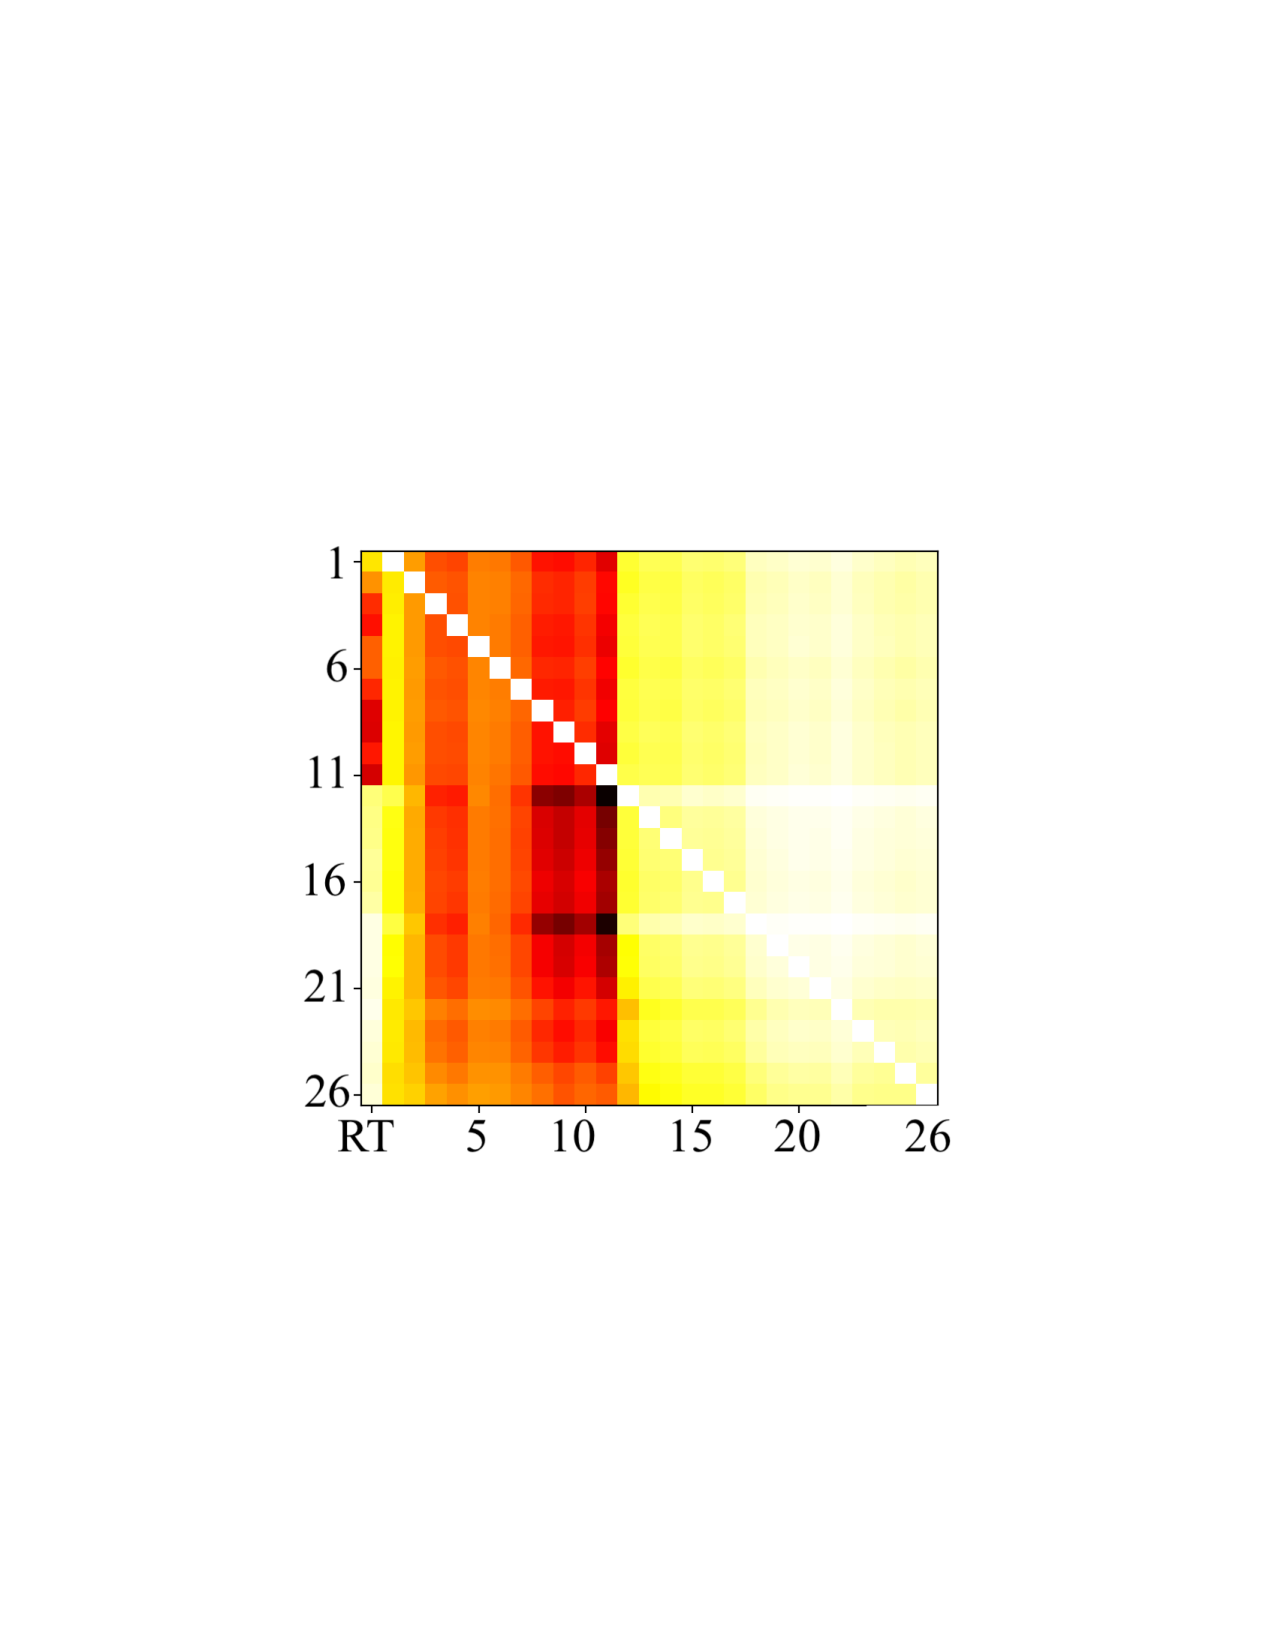
\includegraphics[width=0.4\textwidth, height=50mm]{plots/heatmap_writing.pdf}}}\\
     \\
     Dependency tree: RT: [8, 9, 11], 9: [26], 11: [1, 2, 3, 4, 5, 6, 7, 10, 12, 13, 14, 15, 16, 17, 18, 19, 20, 21, 22, 23, 24, 25] \\
     \begin{enumerate}[topsep=-5pt, noitemsep,leftmargin=*]
      \item One week after an outbreak of Legionnaires ' disease at a Manhattan hospital was blamed for the death of a patient , a second medical center , Harlem Hospital Center , a few miles away , announced yesterday that it might have identified traces of the bacteria in one of its buildings 
      \item The bacteria have now been detected in as many as three city hospital buildings in two months , highlighting what experts said was a barely visible but potentially deadly problem plaguing hospitals in the city \end{enumerate}\\
     \vspace{-2.6em}$\ldots$\\
     \vspace{-2.3em}
     \begin{enumerate}[topsep=-5pt, noitemsep,leftmargin=*]
     \setcounter{enumi}{6}
      \item Two of those patients later died , and an autopsy on one showed last week that Legionnaires ' disease had been the cause 
      \item \uline{On the same day that NewYork Presbyterian announced the results , the hospital disclosed that the water supply at a second building that it operates , the Greenberg Pavilion , on the Upper East Side , had also tested positive for the bacteria , though no cases have been diagnosed} 
      \item \uline{According to the Centers for Disease Control and Prevention , up to 18,000 people in the United States contract Legionnaires ' disease each year , though it is rarely deadly unless those infected have weakened immune systems} 
      \item The bacteria that causes it , which first became widely known in the United States after a large outbreak at a Philadelphia hotel in 1976 , are almost always present in the city 's water supply 
      \item \uline{Hospitals are particularly vulnerable to outbreaks} 
      \item But Dr Victor Yu , the chief of infectious diseases at the Pittsburgh Veterans Administration Health Care center , who is an expert on Legionnaires ' disease , said that few test their water supplies routinely \end{enumerate}\\
      \vspace{-2.4em}$\ldots$\\
      \vspace{-2em}
     \begin{enumerate}[topsep=-5pt, noitemsep,leftmargin=*]
     \setcounter{enumi}{17}
      \item  One expert on Legionnaires ' disease , Dr Joseph S UNK , a professor of clinical medicine and pediatrics at Albert Einstein College of Medicine , said he would not be surprised if other hospitals came forward as well 
      \end{enumerate}\\
      \vspace{-2.4em}$\ldots$\\
      \vspace{-2em}
     \begin{enumerate}[topsep=-5pt, noitemsep,leftmargin=*]
     \setcounter{enumi}{25}
      \item `` If I 'm working here and something is in the water , I have to be careful , '' he said \vspace{-1.2em}
      \end{enumerate}\\
      \bottomrule
      \end{tabular}
      \caption{Example of attention scores, derived dependency tree and text for a test sentence in the Writing Quality dataset (gold label=very good). Root sentences are underlined. In this example, the beginning of the document is likely to be the root.}
      \label{tab:latent_writing}
      \end{center}
      \end{table}
\end{landscape}

\begin{table}[h!]
     \begin{center}
     \begin{tabular}{cllll|l}
     \toprule
                          &     & Yelp 2017      & Congressional Votes & Writing Quality & GUM\\ \hline\hline
\multicolumn{2}{l}{Tree height} & 2.253          & 2.162               & 3.162 &101.5          \\ \hline
\multirow{12}{*}{Nodes}   & 1   & 12.58\%        & 14.59\%             & 10.54\%    &1.57\%     \\
                          & 2   & 74.15\%        & 79.36\%             & 57.4\%    & \textless{}1\%     \\
                          & 3   & 12.51\%        & 5.80\%              & 18.4\%   &1.62\%       \\
                          & 4   & \textless{}1\% & \textless{}1\%      & 7.41\%    &3.21\%      \\
                          & 5   & \textless{}1\% & 0                   & 3.16\%   &2.62\%       \\
                          & 6   & \textless{}1\% & 0                   & 1.5\%   &1.42\%        \\
                          & 7   & 0              & 0                   & 1.09\%  &2.97\%        \\
                          & 8   & 0              & 0                   & \textless{}1\% &2.06\% \\
                          & 9   & 0              & 0                   & \textless{}1\% &2.64\% \\
                          & 10  & 0              & 0                   & \textless{}1\% &1.82\% \\
                          & 11  & 0              & 0                   & \textless{}1\% &1.93\% \\
                          & 12  & 0              & 0                   & \textless{}1\% &2.25\%\\
                & 13 & 0 &0 &0 &1.19\%\\
                &\ldots & \ldots & \ldots & \ldots &\ldots \\
                & 109 & 0 &0 &0 &\textless{}1\%\\
                \bottomrule
                          
\end{tabular}
      \caption{Average tree height and percentage of nodes at each depth of the tree for the derived dependency trees. For the GUM corpus, the dependency trees are derived from the gold-labeled RST trees.}
      \label{tab:latent_trees}
      \end{center}
      \end{table}
      
\smallskip
\noindent\textbf{Dependency Trees} We provide a quantitative analysis in Table \ref{tab:latent_trees} to support the observations made in the previous section. For reference, we include statistics for dependency trees that are instead derived from RST trees on the GUM corpus \cite{Zeldes:2017}.\footnote{We choose to analyze this corpus (instead of RST-DT) because it encompasses several genres beyond just news (interviews, travel guides, how-to guides, academic writing, biographies, fiction) and serves as a better point of comparison for the three datasets.} While RST dependency trees are expected to be deeper in part because they are at the EDU instead of sentence-level, we also note they are not as top-heavy with a more even distribution of nodes at different depths. As surmised earlier, the trees on Yelp are very shallow, consistent with results in \newcite{Liu:2018}. However, our shallow trees on the Congressional Votes are not consistent with the deeper trees found by \newcite{Liu:2018}. We speculate we may have trained longer (explaining the better accuracy) and the model may have learned better trees for the task. The only task achieving deeper trees is that of identifying very good writing.  

\smallskip
\noindent\textbf{Root Sentences} Because the trees are so shallow, we analyze the root sentences in more depth to confirm our suspicions of lexical cues. We calculate the positive pointwise mutual information scores for a root word occurring in the root sentence as compared to all other sentences. Our results are listed in Table \ref{tab:latent_ppmi}.
\begin{table}[h!]
     \begin{center}
     \begin{tabular}{lp{10cm}}
\toprule
Yelp                & uuu, sterne, star, rating, deduct, 0, edit, underwhelmed, update, allgemein \\ 
Congressional Votes & oppose, republican, majority, thank, gentleman, leadership, california, measure, president, vote    \\ 
Writing Quality     & valley, mp3, firm, capital, universal, venture, silicon, analyst, capitalist, street        \\ \bottomrule
\end{tabular}
\caption{Top 10 words most associated with the root sentence (measured with PPMI).}
      \label{tab:latent_ppmi}
      \end{center}
      \end{table}
      
In the Yelp dataset, words in the root sentence can express sentiment (\lit{underwhelmed}), but also reflect cases where a Yelper explicitly mentions how many stars (\lit{sterne} in German) they are going to give (\lit{0}). The model interestingly learns the idiosyncratic rating system of a particularly prolific Yelper who uses \lit{uuu} to symbolize a star. While we do find sentiment-bearing words\footnote{Sentiment scores were calculated using the model in \newcite{Hutto:2014}, as packaged in NLTK.} to occur on average more frequently in the root sentence as compared to other sentences, this difference is marginally significant (t-test, p=0.057). This result suggests that more than just sentiment is being learned, as confirmed by the many non-sentiment words found in the word association list.

For the Congressional Votes, the list contains words that explicitly express their opinion (\lit{oppose}) but also politeness (\lit{thank}) and other terms used for stance-taking.

The list for Writing Quality revolves around tech, suggesting the model may be learning topics instead of actual good or bad writing. The topics were not controlled for and warrants further research into the validity of the dataset.

As a final analysis of root sentences, we implement the \textbf{root-only} model for the Yelp dataset, where we prune the original dataset to include only the root sentences. We hypothesize the \textbf{baseline} model only attends to the root sentences and thus expect this model to perform comparably to the original. However, as illustrated in Table \ref{tab:latent_accuracy_variants}, the accuracy drops considerably. Although this is a negative result, we understand this is likely because the biLSTM is making use of all the sentences, such that the structured attention does not have to. This observation guides our design decision to remove the biLSTM for the \textbf{deeper} model. 

\begin{table}[t]
\centering
\begin{tabular}{ll}
\toprule
Model &Yelp 2017 \\\hline \hline 
baseline &71.24  \\
root-only &56.19 \\
edu &70.73\\
deeper &71.04 \\
\bottomrule
\end{tabular}
\caption{Accuracy on sentiment analysis using the baseline \newcite{Liu:2018} and its variants.}
\label{tab:latent_accuracy_variants}
\end{table}

In summary, we found the model learns to identify lexical cues that benefit the task, and in the case of Writing Quality, possibly topics. This finding, together with the mostly shallow trees, leads us to conclude the model is not learning discourse.
 
\section{Can we inject explicit discourse?}
In this section, we attempt to encourage the model to learn structures more similar to RST discourse trees. As a first and straightforward step, we feed in EDUs instead of sentences in the \textbf{edu} model. While performance degrades slightly (see Table \ref{tab:latent_accuracy_variants}), we do not find the resulting dependency trees to be much different, as illustrated in \ref{tab:latent_treevariants}. The average tree height is 2.365 (compared to 2.253) and nodes of depth 3 are only slightly more numerous (14.33\% vs. 12.51\%). We again attribute this to the presence of the biLSTM and other factors we attempt to address in the \textbf{deeper} model. In future work, we intend to re-evaluate this model \emph{after} making the changes to the network mentioned in the \textbf{deeper} model, to more fairly assess the impact of EDU-level inputs, and additionally evaluate on the other two tasks. 

\section{Can we learn deeper structures?} 
\begin{table}[t]
     \begin{center}
     \begin{tabular}{cllll}
     \toprule
                          &     & baseline   & edu & deeper \\ \hline\hline
\multicolumn{2}{l}{Tree height} & 2.253          & 2.365              &2.803           \\ \hline
\multirow{7}{*}{Nodes}   & 1   & 12.58\%        & 9.79\%             & 15.67\%         \\
                          & 2   & 74.15\%        & 74.16\%             & 51.9\%          \\
                          & 3   & 12.51\%        & 14.33\%              & 26.25\%          \\
                          & 4   & \textless{}1\% & \textless{}1\%      & 5.43\%          \\
                          & 5   & \textless{}1\% & \textless{}1\%                   & \textless{}1\%          \\
                          & 6   & \textless{}1\% & \textless{}1\%                   & \textless{}1\%           \\
                          & 7   & 0              & \textless{}1\%                   & \textless{}1\%        \\
                \bottomrule
                          
\end{tabular}
      \caption{Average tree height and percentage of nodes at each depth of the tree for the baseline model and its variants.}
      \label{tab:latent_treevariants}
      \end{center}
      \end{table}
      
We have seen that the \textbf{baseline} and \textbf{edu} models do not learn deep structures and the structured attention seems to attend mainly to the root sentence. Here we attempt to address these shortcomings by implementing the \textbf{deeper} model (due to resource constraints, we evaluate only on Yelp 2017). This model removes the document-level biLSTM to place the burden on the structured attention for composing sentences. We additionally take into account information from the subtrees for the structured attention and use a sum weighted by the root scores in the pooling layer. The performance degrades slightly (see Table\ref{tab:latent_accuracy_variants}), but critically the model learns deeper trees, as can be seen in Table \ref{tab:latent_treevariants}. The average height is 2.803 (compared to 2.253) and there are considerably more nodes of depth 3 and 4.

A possibility we must consider is that these tasks don't require deeper structures. That is, there are sufficient patterns in the words of a sentence that don't necessitate composition over sentences. This is quite possible for sentiment analysis and Congressional debates prediction, as evidenced by the clear patterns we find in the texts. The challenge then is to find a task that is not susceptible to these pitfalls, but is also tractable for an NLP setting.

\section{Chapter Summary}

In this chapter, we performed a detailed analysis of the model in \newcite{Liu:2018}, and several proposed variants of it. We were motivated by two questions: what is the model learning, and is it discourse? To answer these questions we analyzed the attention scores, the derived dependency trees and words in the root sentences. This analysis revealed that the model mostly attended to the root sentences, and specifically lexical cues that were helpful to each task. There was no discernible discourse in these structures. This finding prompted our next question of whether we could inject explicit structure. This model also failed to yield discourse-like structures, which prompted our next question. How can we induce deeper structures? We made a series of changes to the model to remove artifacts that were trying to take on duties of the structured attention, such as the biLSTM. We succeeded in showing that we could achieve deeper dependency trees, although we would not yet consider these to represent discourse. We speculate the tasks themselves do not require knowledge of discourse. Our challenge for future work is then to find a new task that makes more use of discourse. 

This study opens many avenues of research to further explore latent representations of discourse, combined with explicit structure. In particular, the attention scores could be hard-wired to reflect the structure of the corresponding RST tree. These explicit structures could also be used just for initialization, then allowing the model to learn a derivative structure.

\chapter{Conclusion}
\label{ch:conclusion}

In this report, we focused on the one hand on discourse as dictated by a specific linguistic theory (RST), and on the other hand on discourse purportedly learned by a model. 

Our first study investigated segmentation of RST discourse units in the medical domain. We present a first, small-scale corpus of medical documents annotated with EDUs. Errors in the medical domain provide insights into the differences at lower linguistic levels for this domain, and suggest possible problem areas with the operationalization of RST.

Our second study explored the model of \newcite{Liu:2018} that claims to learn discourse structures by using structured attention that parses into a dependency tree. A careful analysis reveals the structures are not discourse and instead shows the model mostly learns lexical cues. We propose a variant of the model that is able to induce deeper structures on the task of sentiment analysis.

\section{Future Work}
In future work, we would like to understand whether errors in discourse segmentation, which undoubtedly affect the discourse trees, have a detectable effect on a downstream task. 

For our analysis of latent structures, we would like to understand whether deeper structures can be induced on the other tasks, as well. More broadly, we would like to explore other tasks such as essay scoring or argumentation mining that purportedly make more use of discourse.





\clearpage
\phantomsection
\addcontentsline {toc}{chapter}{\bibname}  %% Force Bibliography to appear in contents
\singlespace
\bibliographystyle{utthesis2015}
\bibliography{refs}

%\begin{thesisauthorvita}
% Stephen Roller was born in the early hours of a winter's day in 1988 in
% Baltimore, Maryland. He spent his formative years in Charlotte, North
% Carolina. He obtained a Bachelors of Science in Computer Science from
% North Carolina State University in 2010, and then entered graduate school
% at the University of Texas at Austin. He obtained a Masters of Science in
% Computer Science in 2014, and continued his doctoral studies, where he
% has been working on natural language understanding.
%\end{thesisauthorvita}

\end{document}
